% Options for packages loaded elsewhere
\PassOptionsToPackage{unicode}{hyperref}
\PassOptionsToPackage{hyphens}{url}
%
\documentclass[
  ignorenonframetext,
]{beamer}
\usepackage{pgfpages}
\setbeamertemplate{caption}[numbered]
\setbeamertemplate{caption label separator}{: }
\setbeamercolor{caption name}{fg=normal text.fg}
\beamertemplatenavigationsymbolsempty
% Prevent slide breaks in the middle of a paragraph
\widowpenalties 1 10000
\raggedbottom
\setbeamertemplate{part page}{
  \centering
  \begin{beamercolorbox}[sep=16pt,center]{part title}
    \usebeamerfont{part title}\insertpart\par
  \end{beamercolorbox}
}
\setbeamertemplate{section page}{
  \centering
  \begin{beamercolorbox}[sep=12pt,center]{part title}
    \usebeamerfont{section title}\insertsection\par
  \end{beamercolorbox}
}
\setbeamertemplate{subsection page}{
  \centering
  \begin{beamercolorbox}[sep=8pt,center]{part title}
    \usebeamerfont{subsection title}\insertsubsection\par
  \end{beamercolorbox}
}
\AtBeginPart{
  \frame{\partpage}
}
\AtBeginSection{
  \ifbibliography
  \else
    \frame{\sectionpage}
  \fi
}
\AtBeginSubsection{
  \frame{\subsectionpage}
}
\usepackage{amsmath,amssymb}
\usepackage{iftex}
\ifPDFTeX
  \usepackage[T1]{fontenc}
  \usepackage[utf8]{inputenc}
  \usepackage{textcomp} % provide euro and other symbols
\else % if luatex or xetex
  \usepackage{unicode-math} % this also loads fontspec
  \defaultfontfeatures{Scale=MatchLowercase}
  \defaultfontfeatures[\rmfamily]{Ligatures=TeX,Scale=1}
\fi
\usepackage{lmodern}
\ifPDFTeX\else
  % xetex/luatex font selection
\fi
% Use upquote if available, for straight quotes in verbatim environments
\IfFileExists{upquote.sty}{\usepackage{upquote}}{}
\IfFileExists{microtype.sty}{% use microtype if available
  \usepackage[]{microtype}
  \UseMicrotypeSet[protrusion]{basicmath} % disable protrusion for tt fonts
}{}
\makeatletter
\@ifundefined{KOMAClassName}{% if non-KOMA class
  \IfFileExists{parskip.sty}{%
    \usepackage{parskip}
  }{% else
    \setlength{\parindent}{0pt}
    \setlength{\parskip}{6pt plus 2pt minus 1pt}}
}{% if KOMA class
  \KOMAoptions{parskip=half}}
\makeatother
\usepackage{xcolor}
\newif\ifbibliography
\usepackage{color}
\usepackage{fancyvrb}
\newcommand{\VerbBar}{|}
\newcommand{\VERB}{\Verb[commandchars=\\\{\}]}
\DefineVerbatimEnvironment{Highlighting}{Verbatim}{commandchars=\\\{\}}
% Add ',fontsize=\small' for more characters per line
\usepackage{framed}
\definecolor{shadecolor}{RGB}{248,248,248}
\newenvironment{Shaded}{\begin{snugshade}}{\end{snugshade}}
\newcommand{\AlertTok}[1]{\textcolor[rgb]{0.94,0.16,0.16}{#1}}
\newcommand{\AnnotationTok}[1]{\textcolor[rgb]{0.56,0.35,0.01}{\textbf{\textit{#1}}}}
\newcommand{\AttributeTok}[1]{\textcolor[rgb]{0.13,0.29,0.53}{#1}}
\newcommand{\BaseNTok}[1]{\textcolor[rgb]{0.00,0.00,0.81}{#1}}
\newcommand{\BuiltInTok}[1]{#1}
\newcommand{\CharTok}[1]{\textcolor[rgb]{0.31,0.60,0.02}{#1}}
\newcommand{\CommentTok}[1]{\textcolor[rgb]{0.56,0.35,0.01}{\textit{#1}}}
\newcommand{\CommentVarTok}[1]{\textcolor[rgb]{0.56,0.35,0.01}{\textbf{\textit{#1}}}}
\newcommand{\ConstantTok}[1]{\textcolor[rgb]{0.56,0.35,0.01}{#1}}
\newcommand{\ControlFlowTok}[1]{\textcolor[rgb]{0.13,0.29,0.53}{\textbf{#1}}}
\newcommand{\DataTypeTok}[1]{\textcolor[rgb]{0.13,0.29,0.53}{#1}}
\newcommand{\DecValTok}[1]{\textcolor[rgb]{0.00,0.00,0.81}{#1}}
\newcommand{\DocumentationTok}[1]{\textcolor[rgb]{0.56,0.35,0.01}{\textbf{\textit{#1}}}}
\newcommand{\ErrorTok}[1]{\textcolor[rgb]{0.64,0.00,0.00}{\textbf{#1}}}
\newcommand{\ExtensionTok}[1]{#1}
\newcommand{\FloatTok}[1]{\textcolor[rgb]{0.00,0.00,0.81}{#1}}
\newcommand{\FunctionTok}[1]{\textcolor[rgb]{0.13,0.29,0.53}{\textbf{#1}}}
\newcommand{\ImportTok}[1]{#1}
\newcommand{\InformationTok}[1]{\textcolor[rgb]{0.56,0.35,0.01}{\textbf{\textit{#1}}}}
\newcommand{\KeywordTok}[1]{\textcolor[rgb]{0.13,0.29,0.53}{\textbf{#1}}}
\newcommand{\NormalTok}[1]{#1}
\newcommand{\OperatorTok}[1]{\textcolor[rgb]{0.81,0.36,0.00}{\textbf{#1}}}
\newcommand{\OtherTok}[1]{\textcolor[rgb]{0.56,0.35,0.01}{#1}}
\newcommand{\PreprocessorTok}[1]{\textcolor[rgb]{0.56,0.35,0.01}{\textit{#1}}}
\newcommand{\RegionMarkerTok}[1]{#1}
\newcommand{\SpecialCharTok}[1]{\textcolor[rgb]{0.81,0.36,0.00}{\textbf{#1}}}
\newcommand{\SpecialStringTok}[1]{\textcolor[rgb]{0.31,0.60,0.02}{#1}}
\newcommand{\StringTok}[1]{\textcolor[rgb]{0.31,0.60,0.02}{#1}}
\newcommand{\VariableTok}[1]{\textcolor[rgb]{0.00,0.00,0.00}{#1}}
\newcommand{\VerbatimStringTok}[1]{\textcolor[rgb]{0.31,0.60,0.02}{#1}}
\newcommand{\WarningTok}[1]{\textcolor[rgb]{0.56,0.35,0.01}{\textbf{\textit{#1}}}}
\usepackage{graphicx}
\makeatletter
\def\maxwidth{\ifdim\Gin@nat@width>\linewidth\linewidth\else\Gin@nat@width\fi}
\def\maxheight{\ifdim\Gin@nat@height>\textheight\textheight\else\Gin@nat@height\fi}
\makeatother
% Scale images if necessary, so that they will not overflow the page
% margins by default, and it is still possible to overwrite the defaults
% using explicit options in \includegraphics[width, height, ...]{}
\setkeys{Gin}{width=\maxwidth,height=\maxheight,keepaspectratio}
% Set default figure placement to htbp
\makeatletter
\def\fps@figure{htbp}
\makeatother
\setlength{\emergencystretch}{3em} % prevent overfull lines
\providecommand{\tightlist}{%
  \setlength{\itemsep}{0pt}\setlength{\parskip}{0pt}}
\setcounter{secnumdepth}{-\maxdimen} % remove section numbering
\ifLuaTeX
  \usepackage{selnolig}  % disable illegal ligatures
\fi
\IfFileExists{bookmark.sty}{\usepackage{bookmark}}{\usepackage{hyperref}}
\IfFileExists{xurl.sty}{\usepackage{xurl}}{} % add URL line breaks if available
\urlstyle{same}
\hypersetup{
  pdftitle={Descriptive-Analysis-Union-Density--Trade-Union-DB-.R},
  pdfauthor={pretender},
  hidelinks,
  pdfcreator={LaTeX via pandoc}}

\title{Descriptive-Analysis-Union-Density--Trade-Union-DB-.R}
\author{pretender}
\date{2023-12-26}

\begin{document}
\frame{\titlepage}

\begin{frame}[fragile]
\begin{Shaded}
\begin{Highlighting}[]
\FunctionTok{library}\NormalTok{(hrbrthemes)}

\CommentTok{\# Descriptive statistics}
\NormalTok{summary\_stats }\OtherTok{\textless{}{-}}\NormalTok{ trade\_union\_density }\SpecialCharTok{\%\textgreater{}\%}
  \FunctionTok{summarise}\NormalTok{(}
    \AttributeTok{Mean =} \FunctionTok{mean}\NormalTok{(Value, }\AttributeTok{na.rm =} \ConstantTok{TRUE}\NormalTok{),}
    \AttributeTok{Median =} \FunctionTok{median}\NormalTok{(Value, }\AttributeTok{na.rm =} \ConstantTok{TRUE}\NormalTok{),}
    \AttributeTok{SD =} \FunctionTok{sd}\NormalTok{(Value, }\AttributeTok{na.rm =} \ConstantTok{TRUE}\NormalTok{)}
\NormalTok{  )}
\FunctionTok{print}\NormalTok{(summary\_stats)}
\end{Highlighting}
\end{Shaded}

\begin{verbatim}
## # A tibble: 1 x 3
##    Mean Median    SD
##   <dbl>  <dbl> <dbl>
## 1  27.7   19.7  20.6
\end{verbatim}

\begin{Shaded}
\begin{Highlighting}[]
\NormalTok{ftheme }\OtherTok{\textless{}{-}} \FunctionTok{theme}\NormalTok{(}
  \AttributeTok{plot.title =} \FunctionTok{element\_text}\NormalTok{(}\AttributeTok{size =} \DecValTok{25}\NormalTok{),}
  \AttributeTok{axis.title =} \FunctionTok{element\_text}\NormalTok{(}\AttributeTok{size =} \DecValTok{20}\NormalTok{),}
  \AttributeTok{axis.text.x =} \FunctionTok{element\_text}\NormalTok{(}\AttributeTok{size =} \DecValTok{15}\NormalTok{),}
  \AttributeTok{axis.text.y =} \FunctionTok{element\_text}\NormalTok{(}\AttributeTok{size =} \DecValTok{15}\NormalTok{)}
\NormalTok{)}
\CommentTok{\# Histogram of Union Density}
\NormalTok{d1 }\OtherTok{\textless{}{-}} \FunctionTok{ggplot}\NormalTok{(trade\_union\_density, }\FunctionTok{aes}\NormalTok{(}\AttributeTok{x =}\NormalTok{ Value)) }\SpecialCharTok{+}
  \FunctionTok{geom\_histogram}\NormalTok{(}\AttributeTok{bins =} \DecValTok{30}\NormalTok{, }\AttributeTok{fill =} \StringTok{"\#69b3a2"}\NormalTok{, }\AttributeTok{color =} \StringTok{"black"}\NormalTok{) }\SpecialCharTok{+}
  \FunctionTok{labs}\NormalTok{(}
    \AttributeTok{title =} \StringTok{"Histogram of Union Density"}\NormalTok{,}
    \AttributeTok{x =} \StringTok{"Union Density in(\%)"}\NormalTok{,}
    \AttributeTok{y =} \StringTok{"Frequency"}
\NormalTok{  ) }\SpecialCharTok{+}
\NormalTok{  ftheme}
\FunctionTok{print}\NormalTok{(d1)}
\end{Highlighting}
\end{Shaded}

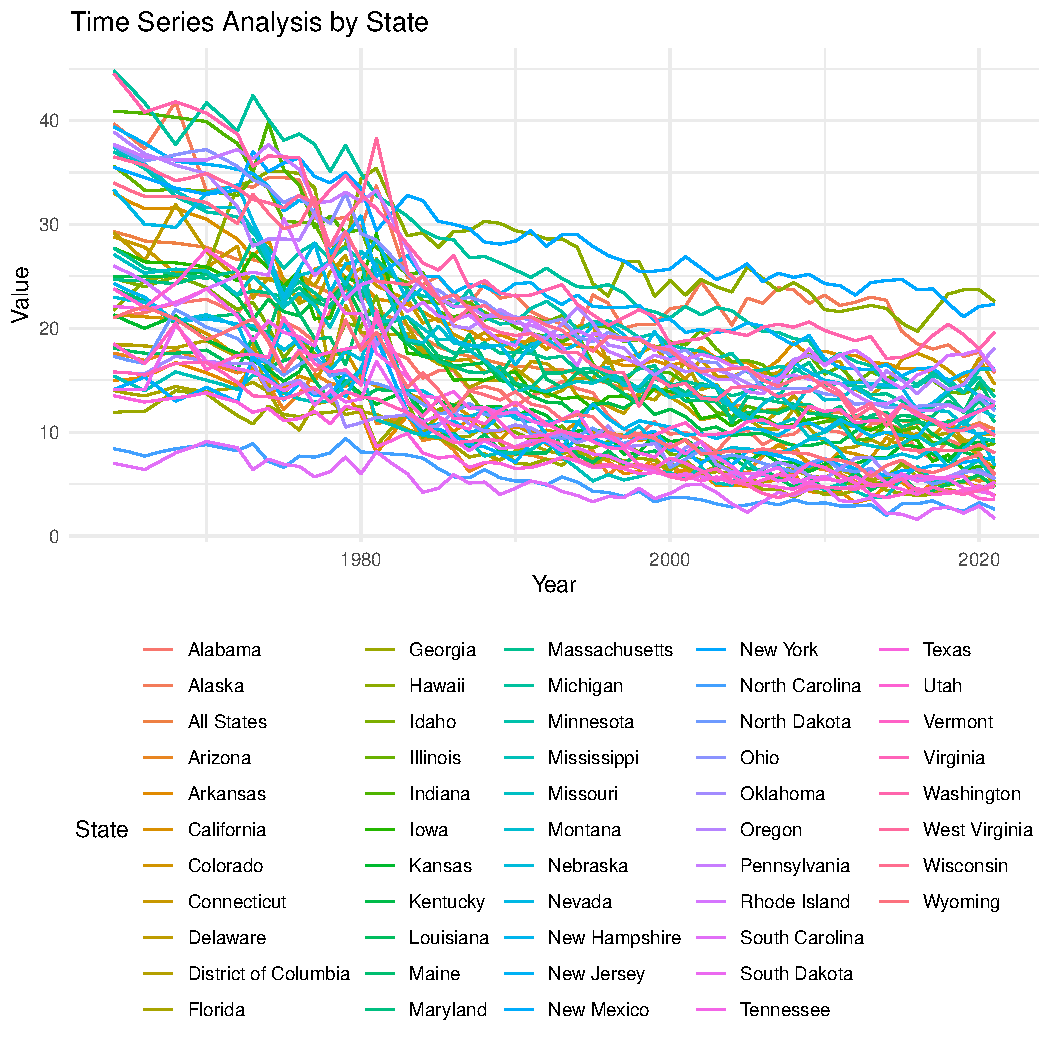
\includegraphics{Descriptive-Analysis-Union-Density--Trade-Union-DB-_files/figure-beamer/unnamed-chunk-1-1.pdf}

\begin{Shaded}
\begin{Highlighting}[]
\CommentTok{\# Union Density is right{-}skewed,}
\CommentTok{\# it would suggest that most countries have a lower union}
\CommentTok{\# density, but a few countries have a very high union density. The peak of the}
\CommentTok{\# histogram would indicate the most common range of union density. If there are}
\CommentTok{\# any gaps or isolated bars, they might indicate outliers or special cases.}
\CommentTok{\# remember, a histogram is a tool for exploring your data. It provides a visual}
\CommentTok{\# summary that can guide further analysis, but it\textquotesingle{}s always important to consider}
\CommentTok{\# other factors and context related to your data.}




\CommentTok{\# Histogram workplace\_rights}
\NormalTok{d2 }\OtherTok{\textless{}{-}} \FunctionTok{ggplot}\NormalTok{(workplace\_rights, }\FunctionTok{aes}\NormalTok{(}\AttributeTok{x =}\NormalTok{ obs\_value)) }\SpecialCharTok{+}
  \FunctionTok{geom\_histogram}\NormalTok{(}\AttributeTok{bins =} \DecValTok{30}\NormalTok{, }\AttributeTok{fill =} \StringTok{"blue"}\NormalTok{, }\AttributeTok{color =} \StringTok{"black"}\NormalTok{) }\SpecialCharTok{+}
  \FunctionTok{labs}\NormalTok{(}
    \AttributeTok{title =} \StringTok{"Histogram of National Complianance with International Law (ILO)"}\NormalTok{,}
    \AttributeTok{x =} \StringTok{"Workplace Rights Complianace with International Law"}\NormalTok{,}
    \AttributeTok{y =} \StringTok{"Frequency"}
\NormalTok{  ) }\SpecialCharTok{+}
\NormalTok{  ftheme}
\FunctionTok{print}\NormalTok{(d2)}
\end{Highlighting}
\end{Shaded}

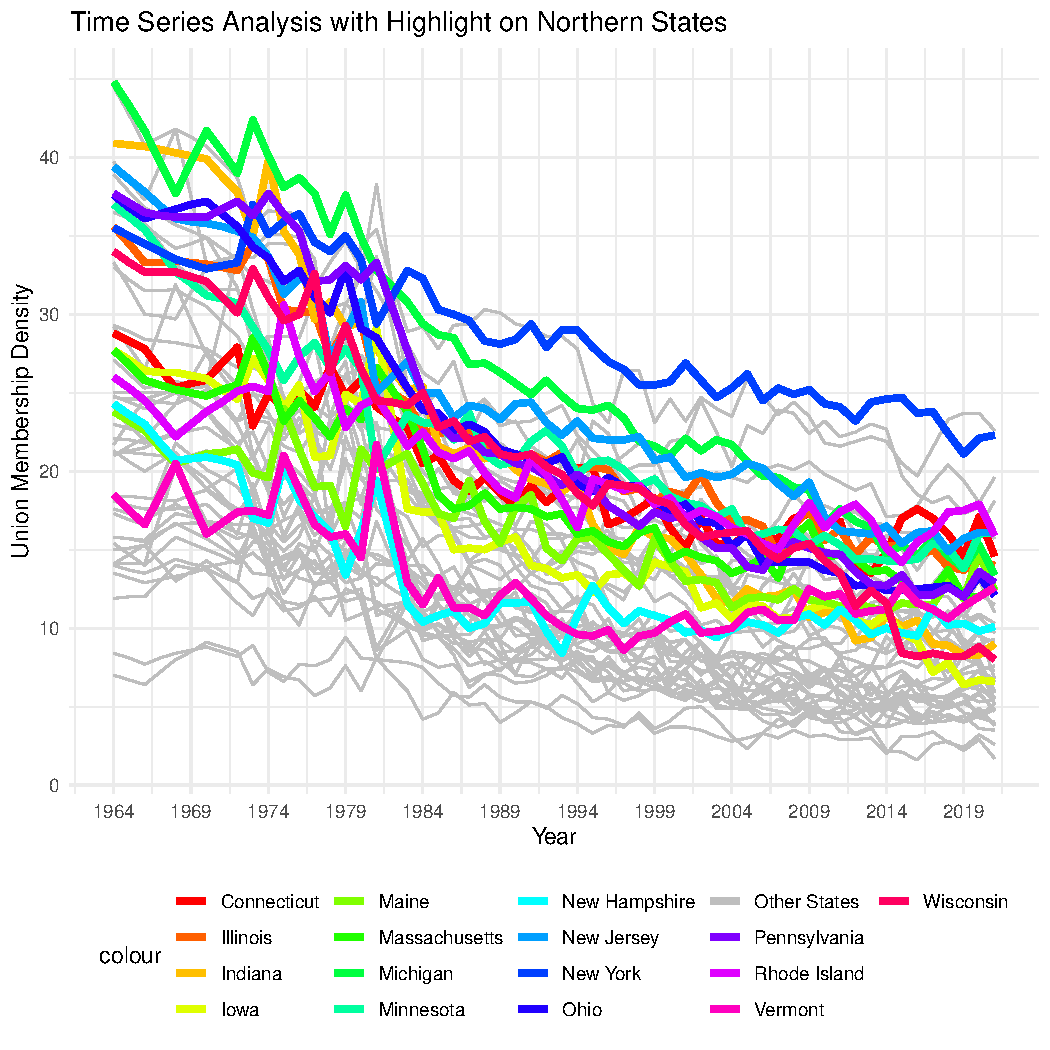
\includegraphics{Descriptive-Analysis-Union-Density--Trade-Union-DB-_files/figure-beamer/unnamed-chunk-1-2.pdf}

\begin{Shaded}
\begin{Highlighting}[]
\NormalTok{d3 }\OtherTok{\textless{}{-}} \FunctionTok{ggplot}\NormalTok{(cbcr, }\FunctionTok{aes}\NormalTok{(}\AttributeTok{x =}\NormalTok{ obs\_value)) }\SpecialCharTok{+}
  \FunctionTok{geom\_histogram}\NormalTok{(}\AttributeTok{bins =} \DecValTok{30}\NormalTok{, }\AttributeTok{fill =} \StringTok{"\#404080"}\NormalTok{, }\AttributeTok{color =} \StringTok{"black"}\NormalTok{) }\SpecialCharTok{+}
  \FunctionTok{labs}\NormalTok{(}
    \AttributeTok{title =} \StringTok{"Histogram of National Collective Bargaining Coverage"}\NormalTok{,}
    \AttributeTok{x =} \StringTok{"Collective Bargaining Coverage"}\NormalTok{,}
    \AttributeTok{y =} \StringTok{"Frequency"}
\NormalTok{  ) }\SpecialCharTok{+}
\NormalTok{  ftheme}
\FunctionTok{print}\NormalTok{(d3)}
\end{Highlighting}
\end{Shaded}

\includegraphics{Descriptive-Analysis-Union-Density--Trade-Union-DB-_files/figure-beamer/unnamed-chunk-1-3.pdf}

\begin{Shaded}
\begin{Highlighting}[]
\DocumentationTok{\#\#\#\#                                                    frequency tables to be added to to the Wiki}
\CommentTok{\# Assuming trade\_union\_density is your data frame and it}
\CommentTok{\# has columns named \textquotesingle{}Country\textquotesingle{} and \textquotesingle{}Value\textquotesingle{}}
\NormalTok{US\_UnionDensity }\OtherTok{\textless{}{-}}\NormalTok{ trade\_union\_density }\SpecialCharTok{\%\textgreater{}\%}
  \FunctionTok{filter}\NormalTok{(Country }\SpecialCharTok{==} \StringTok{"United States"}\NormalTok{) }\SpecialCharTok{\%\textgreater{}\%}
  \FunctionTok{summarize}\NormalTok{(}\AttributeTok{UnionDensityValue =} \FunctionTok{mean}\NormalTok{(Value)) }\SpecialCharTok{\%\textgreater{}\%}
\NormalTok{  .}\SpecialCharTok{$}\NormalTok{UnionDensityValue }\CommentTok{\# Extracting the numeric value}
\CommentTok{\# Calculate the median of the Union Density}
\NormalTok{Median\_UnionDensity }\OtherTok{\textless{}{-}} \FunctionTok{median}\NormalTok{(trade\_union\_density}\SpecialCharTok{$}\NormalTok{Value)}
\CommentTok{\# Create a data frame for the lines}
\NormalTok{lines\_df }\OtherTok{\textless{}{-}} \FunctionTok{data.frame}\NormalTok{(}
  \AttributeTok{xintercept =} \FunctionTok{c}\NormalTok{(US\_UnionDensity, Median\_UnionDensity),}
  \AttributeTok{line\_id =} \FunctionTok{c}\NormalTok{(}\StringTok{"United States"}\NormalTok{, }\StringTok{"Median"}\NormalTok{)}
\NormalTok{)}
\NormalTok{d1 }\OtherTok{\textless{}{-}} \FunctionTok{ggplot}\NormalTok{(trade\_union\_density, }\FunctionTok{aes}\NormalTok{(}\AttributeTok{x =}\NormalTok{ Value)) }\SpecialCharTok{+}
  \FunctionTok{geom\_histogram}\NormalTok{(}\AttributeTok{bins =} \DecValTok{30}\NormalTok{, }\AttributeTok{fill =} \StringTok{"\#69b3a2"}\NormalTok{, }\AttributeTok{color =} \StringTok{"black"}\NormalTok{) }\SpecialCharTok{+}
  \FunctionTok{geom\_vline}\NormalTok{(}\AttributeTok{data =}\NormalTok{ lines\_df, }\FunctionTok{aes}\NormalTok{(}
    \AttributeTok{xintercept =}\NormalTok{ xintercept,}
    \AttributeTok{linetype =}\NormalTok{ line\_id, }\AttributeTok{color =}\NormalTok{ line\_id}
\NormalTok{  ), }\AttributeTok{size =} \DecValTok{3}\NormalTok{) }\SpecialCharTok{+}
  \FunctionTok{scale\_color\_manual}\NormalTok{(}\AttributeTok{name =} \StringTok{"Line Type"}\NormalTok{, }\AttributeTok{values =} \FunctionTok{c}\NormalTok{(}\StringTok{"United States"} \OtherTok{=} \StringTok{"red"}\NormalTok{, }\StringTok{"Median"} \OtherTok{=} \StringTok{"green"}\NormalTok{)) }\SpecialCharTok{+}
  \FunctionTok{scale\_linetype\_manual}\NormalTok{(}\AttributeTok{name =} \StringTok{"Line Type"}\NormalTok{, }\AttributeTok{values =} \FunctionTok{c}\NormalTok{(}\StringTok{"United States"} \OtherTok{=} \StringTok{"dotted"}\NormalTok{, }\StringTok{"Median"} \OtherTok{=} \StringTok{"dashed"}\NormalTok{)) }\SpecialCharTok{+}
  \FunctionTok{labs}\NormalTok{(}
    \AttributeTok{title =} \StringTok{"Histogram of Union Density"}\NormalTok{,}
    \AttributeTok{x =} \StringTok{"Union Density(in \%)"}\NormalTok{,}
    \AttributeTok{y =} \StringTok{"Frequency"}
\NormalTok{  ) }\SpecialCharTok{+}
\NormalTok{  ftheme }\SpecialCharTok{+}
  \FunctionTok{guides}\NormalTok{(}\AttributeTok{color =} \FunctionTok{guide\_legend}\NormalTok{(}\AttributeTok{override.aes =} \FunctionTok{list}\NormalTok{(}\AttributeTok{linetype =} \FunctionTok{c}\NormalTok{(}\StringTok{"dashed"}\NormalTok{, }\StringTok{"dotted"}\NormalTok{))))}
\FunctionTok{print}\NormalTok{(d1)}
\end{Highlighting}
\end{Shaded}

\includegraphics{Descriptive-Analysis-Union-Density--Trade-Union-DB-_files/figure-beamer/unnamed-chunk-1-4.pdf}

\begin{Shaded}
\begin{Highlighting}[]
\NormalTok{file\_path }\OtherTok{\textless{}{-}}\NormalTok{ (}\StringTok{"\textasciitilde{}/Lab2/graphs/plot\_8{-}1.pdf"}\NormalTok{)}
\FunctionTok{ggsave}\NormalTok{(file\_path, }\AttributeTok{plot =}\NormalTok{ d1)}
\end{Highlighting}
\end{Shaded}

\begin{verbatim}
## Saving 10 x 7 in image
\end{verbatim}

\begin{Shaded}
\begin{Highlighting}[]
\CommentTok{\# Assuming cbcr is your data frame}
\NormalTok{US\_cbcr }\OtherTok{\textless{}{-}}\NormalTok{ cbcr }\SpecialCharTok{\%\textgreater{}\%}
  \FunctionTok{filter}\NormalTok{(ref\_area }\SpecialCharTok{==} \StringTok{"United States"}\NormalTok{) }\SpecialCharTok{\%\textgreater{}\%}
  \FunctionTok{summarize}\NormalTok{(}\AttributeTok{cbcrValue =} \FunctionTok{mean}\NormalTok{(obs\_value)) }\SpecialCharTok{\%\textgreater{}\%}
\NormalTok{  .}\SpecialCharTok{$}\NormalTok{cbcrValue}
\CommentTok{\# Calculate the median of Collective Bargaining Coverage}
\NormalTok{Median\_cbcr }\OtherTok{\textless{}{-}} \FunctionTok{median}\NormalTok{(cbcr}\SpecialCharTok{$}\NormalTok{obs\_value)}
\CommentTok{\# Create a data frame for the lines}
\NormalTok{lines\_df\_cbcr }\OtherTok{\textless{}{-}} \FunctionTok{data.frame}\NormalTok{(}
  \AttributeTok{xintercept =} \FunctionTok{c}\NormalTok{(US\_cbcr, Median\_cbcr),}
  \AttributeTok{line\_id =} \FunctionTok{c}\NormalTok{(}\StringTok{"United States"}\NormalTok{, }\StringTok{"Median"}\NormalTok{)}
\NormalTok{)}
\CommentTok{\# Create histogram for Collective Bargaining Coverage}
\NormalTok{d3 }\OtherTok{\textless{}{-}} \FunctionTok{ggplot}\NormalTok{(cbcr, }\FunctionTok{aes}\NormalTok{(}\AttributeTok{x =}\NormalTok{ obs\_value)) }\SpecialCharTok{+}
  \FunctionTok{geom\_histogram}\NormalTok{(}\AttributeTok{bins =} \DecValTok{30}\NormalTok{, }\AttributeTok{fill =} \StringTok{"\#404080"}\NormalTok{, }\AttributeTok{color =} \StringTok{"black"}\NormalTok{) }\SpecialCharTok{+}
  \FunctionTok{geom\_vline}\NormalTok{(}
    \AttributeTok{data =}\NormalTok{ lines\_df\_cbcr,}
    \FunctionTok{aes}\NormalTok{(}
      \AttributeTok{xintercept =}\NormalTok{ xintercept,}
      \AttributeTok{linetype =}\NormalTok{ line\_id,}
      \AttributeTok{color =}\NormalTok{ line\_id}
\NormalTok{    ),}
    \AttributeTok{size =} \DecValTok{3}
\NormalTok{  ) }\SpecialCharTok{+}
  \FunctionTok{scale\_color\_manual}\NormalTok{(}
    \AttributeTok{name =} \StringTok{"Line Type"}\NormalTok{,}
    \AttributeTok{values =} \FunctionTok{c}\NormalTok{(}
      \StringTok{"United States"} \OtherTok{=} \StringTok{"red"}\NormalTok{,}
      \StringTok{"Median"} \OtherTok{=} \StringTok{"green"}
\NormalTok{    )}
\NormalTok{  ) }\SpecialCharTok{+}
  \FunctionTok{scale\_linetype\_manual}\NormalTok{(}
    \AttributeTok{name =} \StringTok{"Line Type"}\NormalTok{,}
    \AttributeTok{values =} \FunctionTok{c}\NormalTok{(}
      \StringTok{"United States"} \OtherTok{=} \StringTok{"dotted"}\NormalTok{,}
      \StringTok{"Median"} \OtherTok{=} \StringTok{"dashed"}
\NormalTok{    )}
\NormalTok{  ) }\SpecialCharTok{+}
  \FunctionTok{labs}\NormalTok{(}
    \AttributeTok{title =} \StringTok{"Histogram of National Collective Bargaining Coverage"}\NormalTok{,}
    \AttributeTok{x =} \StringTok{"Collective Bargaining Coverage (in \%)"}\NormalTok{,}
    \AttributeTok{y =} \StringTok{"Frequency"}
\NormalTok{  ) }\SpecialCharTok{+}
\NormalTok{  ftheme }\SpecialCharTok{+}
  \FunctionTok{guides}\NormalTok{(}\AttributeTok{color =} \FunctionTok{guide\_legend}\NormalTok{(}\AttributeTok{override.aes =} \FunctionTok{list}\NormalTok{(}\AttributeTok{linetype =} \FunctionTok{c}\NormalTok{(}\StringTok{"dashed"}\NormalTok{, }\StringTok{"dotted"}\NormalTok{))))}
\FunctionTok{print}\NormalTok{(d3)}
\end{Highlighting}
\end{Shaded}

\includegraphics{Descriptive-Analysis-Union-Density--Trade-Union-DB-_files/figure-beamer/unnamed-chunk-1-5.pdf}

\begin{Shaded}
\begin{Highlighting}[]
\NormalTok{file\_path }\OtherTok{\textless{}{-}}\NormalTok{ (}\StringTok{"\textasciitilde{}/Lab2/graphs/plot\_8.pdf"}\NormalTok{)}
\FunctionTok{ggsave}\NormalTok{(file\_path, }\AttributeTok{plot =}\NormalTok{ d3)}
\end{Highlighting}
\end{Shaded}

\begin{verbatim}
## Saving 10 x 7 in image
\end{verbatim}

\begin{Shaded}
\begin{Highlighting}[]
\CommentTok{\# Assuming workplace\_rights is your data frame}
\NormalTok{US\_workplace\_rights }\OtherTok{\textless{}{-}}\NormalTok{ workplace\_rights }\SpecialCharTok{\%\textgreater{}\%}
  \FunctionTok{filter}\NormalTok{(ref\_area }\SpecialCharTok{==} \StringTok{"United States"}\NormalTok{) }\SpecialCharTok{\%\textgreater{}\%}
  \FunctionTok{summarize}\NormalTok{(}\AttributeTok{workplace\_rightsValue =} \FunctionTok{mean}\NormalTok{(obs\_value)) }\SpecialCharTok{\%\textgreater{}\%}
\NormalTok{  .}\SpecialCharTok{$}\NormalTok{workplace\_rightsValue}
\CommentTok{\# Calculate the median of Workplace Rights}
\NormalTok{Median\_workplace\_rights }\OtherTok{\textless{}{-}} \FunctionTok{median}\NormalTok{(workplace\_rights}\SpecialCharTok{$}\NormalTok{obs\_value)}
\CommentTok{\# Create a data frame for the lines}
\NormalTok{lines\_df\_wr }\OtherTok{\textless{}{-}} \FunctionTok{data.frame}\NormalTok{(}
  \AttributeTok{xintercept =} \FunctionTok{c}\NormalTok{(US\_workplace\_rights, Median\_workplace\_rights),}
  \AttributeTok{line\_id =} \FunctionTok{c}\NormalTok{(}\StringTok{"United States"}\NormalTok{, }\StringTok{"Median"}\NormalTok{)}
\NormalTok{)}
\CommentTok{\# Create histogram for Workplace Rights}
\NormalTok{d2 }\OtherTok{\textless{}{-}} \FunctionTok{ggplot}\NormalTok{(workplace\_rights, }\FunctionTok{aes}\NormalTok{(}\AttributeTok{x =}\NormalTok{ obs\_value)) }\SpecialCharTok{+}
  \FunctionTok{geom\_histogram}\NormalTok{(}\AttributeTok{bins =} \DecValTok{30}\NormalTok{, }\AttributeTok{fill =} \StringTok{"blue"}\NormalTok{, }\AttributeTok{color =} \StringTok{"black"}\NormalTok{) }\SpecialCharTok{+}
  \FunctionTok{geom\_vline}\NormalTok{(}
    \AttributeTok{data =}\NormalTok{ lines\_df\_wr,}
    \FunctionTok{aes}\NormalTok{(}\AttributeTok{xintercept =}\NormalTok{ xintercept, }\AttributeTok{linetype =}\NormalTok{ line\_id, }\AttributeTok{color =}\NormalTok{ line\_id), }\AttributeTok{size =} \DecValTok{3}
\NormalTok{  ) }\SpecialCharTok{+}
  \FunctionTok{scale\_color\_manual}\NormalTok{(}
    \AttributeTok{name =} \StringTok{"Line Type"}\NormalTok{,}
    \AttributeTok{values =} \FunctionTok{c}\NormalTok{(}\StringTok{"United States"} \OtherTok{=} \StringTok{"red"}\NormalTok{, }\StringTok{"Median"} \OtherTok{=} \StringTok{"green"}\NormalTok{)}
\NormalTok{  ) }\SpecialCharTok{+}
  \FunctionTok{scale\_linetype\_manual}\NormalTok{(}
    \AttributeTok{name =} \StringTok{"Line Type"}\NormalTok{,}
    \AttributeTok{values =} \FunctionTok{c}\NormalTok{(}\StringTok{"United States"} \OtherTok{=} \StringTok{"dotted"}\NormalTok{, }\StringTok{"Median"} \OtherTok{=} \StringTok{"dashed"}\NormalTok{)}
\NormalTok{  ) }\SpecialCharTok{+}
  \FunctionTok{labs}\NormalTok{(}
    \AttributeTok{title =} \StringTok{"Histogram of National Compliance with International Law (ILO)"}\NormalTok{,}
    \AttributeTok{x =} \StringTok{"Workplace Rights Compliance with International Law (Rating)"}\NormalTok{,}
    \AttributeTok{y =} \StringTok{"Frequency"}
\NormalTok{  ) }\SpecialCharTok{+}
\NormalTok{  ftheme }\SpecialCharTok{+}
  \FunctionTok{guides}\NormalTok{(}\AttributeTok{color =} \FunctionTok{guide\_legend}\NormalTok{(}\AttributeTok{override.aes =} \FunctionTok{list}\NormalTok{(}\AttributeTok{linetype =} \FunctionTok{c}\NormalTok{(}\StringTok{"dashed"}\NormalTok{, }\StringTok{"dotted"}\NormalTok{))))}
\FunctionTok{print}\NormalTok{(d2)}
\end{Highlighting}
\end{Shaded}

\includegraphics{Descriptive-Analysis-Union-Density--Trade-Union-DB-_files/figure-beamer/unnamed-chunk-1-6.pdf}

\begin{Shaded}
\begin{Highlighting}[]
\NormalTok{file\_path }\OtherTok{\textless{}{-}}\NormalTok{ (}\StringTok{"\textasciitilde{}/Lab2/graphs/plot\_9.pdf"}\NormalTok{)}
\FunctionTok{ggsave}\NormalTok{(file\_path, }\AttributeTok{plot =}\NormalTok{ d2)}
\end{Highlighting}
\end{Shaded}

\begin{verbatim}
## Saving 10 x 7 in image
\end{verbatim}
\end{frame}

\end{document}
